% !TEX root = ../notes.tex

\marginnote{\emph{Lecture 5}}[0mm]
We are now going to look at our non-dimensionalised system by looking at the steady states and look at the stability. \\
Previously we just plotted the functions. However, this is slightly harder to do, but we write out, $f(u) = g(u) + h(u) $ and then plot them individually\\\vspace{10pt}
\begin{minipage}{0.45\textwidth}
  \centering
  \begin{tikzpicture}[scale=1.0]
  \begin{axis}[
          axis x line=middle,
          axis y line=middle,
          ymax=1, ymin=0, ylabel=$g(u)$,
          xlabel=$u$
          ]
      \addplot[domain=0:3, blue, ultra thick] {x * (1 - x / 2)};
  \end{axis}
  \end{tikzpicture}
\end{minipage}\hfill
\begin{minipage}{0.45\textwidth}
  \centering
  \begin{tikzpicture}[scale=1.0]
  \begin{axis}[
          axis x line=middle,
          axis y line=middle,
          ymax=1, ymin=0, ylabel=$h(u)$,
          xlabel=$u$
          ]
      \addplot[domain=0:4, blue, ultra thick] {x*x / (1 + x*x)};
  \end{axis}
  \end{tikzpicture}
\end{minipage}\hfill\vspace{10pt}\\
and now we can consider them on the same axis,\\
\begin{figure}[!ht]
\centering
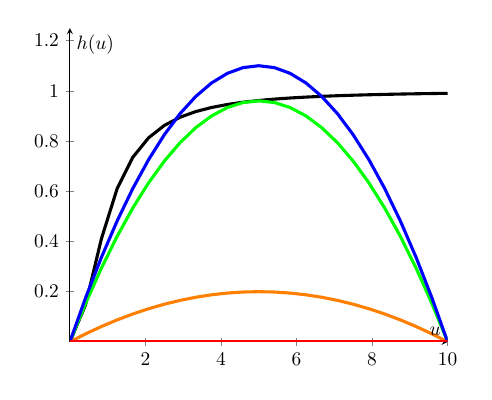
\begin{tikzpicture}[scale=0.7]
\begin{axis}[
        axis x line=middle,
        axis y line=middle,
        ymax=1.25, ymin=0, ylabel=$h(u)$,
        xlabel=$u$
        ]
    \addplot[domain=0:10, black, ultra thick] {1 * x*x / (1 + x*x)};
    \addplot[domain=0:10, green, ultra thick] {1.92/5 * x * (1 - x / 10)};
    \addplot[domain=0:10, orange, ultra thick] {0.4/5 * x * (1 - x / 10)};
    \addplot[domain=0:10, blue, ultra thick] {2.2/5 * x * (1 - x / 10)};
    \addplot[domain=0:10, red, ultra thick] {0};
\end{axis}
\end{tikzpicture}
\end{figure}

Where we can say that there is an equilibrium when $g(u) = 0$ and this is a unstable equilibrium. Now for a $r \ne 0$, then we have the orange curve, then we have that the equilibrium at $0$ is still unstable and there is a new steady state which we find to be stable. We have a third value (green), where we have $u^{**}$, where we have another unstable fixed point. Finally, when we move our function higher again, (blue) and we get a $u^{***}$ that's stable. There is another interesting point, where there is a tangent between the two graphs above this one $u^{**} = u^{***}$ and hence we have three steady states.\\

\noindent
We shall note the geometric approach, we can graph the functions and consider the derivatives around critical points. We can summarise this in a bifurcation diagram.

\subsection{Bifurcation Diagram}
Imagine we have those snapshots and put them on a diagram.
\begin{figure}[!ht]
\centering
\begin{tikzpicture}[scale=1.0]
\begin{axis}[
        ticks = none,
        axis x line=middle,
        axis y line=middle,
        ymax=1.25, ymin=0, ylabel=$u^*$,
        xlabel=$r$
        ]
\end{axis}
\draw (0, 0) circle (0.1);
\draw (1, 0) circle (0.1);
\fill (1, 0.5) circle (0.1);
\draw (2, 0) circle (0.1);
\fill (2, 1) circle (0.1);
\draw (3, 0) circle (0.1);
\fill (3, 1.5) circle (0.1);
\draw (4, 0) circle (0.1);
\fill (4, 2) circle (0.1);
\draw (4, 4) circle (0.1);
\draw (5, 0) circle (0.1);
\fill (5, 2.5) circle (0.1);
\draw (5, 3.5) circle (0.1);
\fill (5, 4.5) circle (0.1);
\draw (6, 0) circle (0.1);
\draw (6, 3) circle (0.1);
\fill (6, 5) circle (0.1);
\node[rotate=80] at (6.5, 5.5) {$\ddots$};
\end{tikzpicture}
\caption{Bifuration Diagram for our system}
\end{figure}
where a filled dot is stable and unfilled is unstable. We can further this by drawing smooth curves along where we have placed the dots and produce said bifurcation diagram. \\

\noindent
Hence, let us think about trajectories of the system. The bifurcation diagram has split us into three different areas. From an initial condition, in a region one (before the unstable area) we have an unstable fixed point and an unstable fixed point. Hence, aslong as you start with a positive initial condition we converge to $u^*$. Moreover, Region 2 is even more interesting, in the unstable area.
\begin{figure}
    \centering
    \begin{minipage}{0.45\textwidth}
        \centering
        \begin{tikzpicture}[scale=1.0]
        \begin{axis}[
                ticks = none,
                axis x line=middle,
                axis y line=middle,
                ymax=3, ymin=0, ylabel=$u(\t)$,
                xlabel=$\t$
                ]
            \addplot[domain=0:3, blue, dotted, ultra thick] {1.5};
        \end{axis}
        \draw [thick] plot [smooth, tension = 1] coordinates { (0, 5) (3, 3.5) (6.8, 3)};
        \draw [thick] plot [smooth, tension = 1] coordinates { (0, 0.3) (3, 2) (6.8, 2.7)};
        \node at (-0.5, 2.9) {\large $u^*$};
        \end{tikzpicture}
        \caption{Steady States of the $R_1$}
    \end{minipage}\hfill
    \begin{minipage}{0.45\textwidth}
        \centering
        \begin{tikzpicture}[scale=1.0]
        \begin{axis}[
                ticks = none,
                axis x line=middle,
                axis y line=middle,
                ymax=3, ymin=0, ylabel=$u(\t)$,
                xlabel=$\t$
                ]
            \addplot[domain=0:3, blue, dotted, ultra thick] {3*1/4};
            \addplot[domain=0:3, blue, dotted, ultra thick] {3*2/4};
            \addplot[domain=0:3, blue, dotted, ultra thick] {3*3/4};
        \end{axis}
        \draw [thick] plot [smooth, tension = 1] coordinates { (0, 5/2) (3, 3.5/2) (6.8, 3/2)};
        \draw [thick] plot [smooth, tension = 1] coordinates { (0, 0.3/2) (3, 2/2) (6.8, 2.7/2)};
        \draw [thick] plot [smooth, tension = 1] coordinates { (0, 5.5) (3, 4.8) (6.8, 4.4)};
        \draw [thick] plot [smooth, tension = 1] coordinates { (0, 3.2) (3, 3.8) (6.8, 4.2)};
        \node at (-0.5, 2.9) {\large $u^{**}$};
        \node at (-0.5, 1.5) {\large $u^*$};
        \node at (-0.5, 4.4) {\large $u^{***}$};
        \end{tikzpicture}
        \caption{Steady States of the $R_1$}
    \end{minipage}
\end{figure}

\marginnote{\emph{Lecture 6}}[0mm]
We can move back to our model. Let $B$ be the population dynamics of predators, and consider $r = \frac{r_B A}{B}$ and consider a slow change in $B$. Consider a decrease in $B$, hence an increase in $r$ and $u$. As soon as you reach an unstable steady state, you jump up to the higher state and carries on as usual.\\


Now we are at a higher level, we have depopulation. So, what happens now as $B$ increases, well then $r$ and $u$ decrease and we follow the branch back down.\\

This phenomena is called Hysteresis. This occurs when the bifurcation diagram has a sudden jump and then a `reason' for the population to decrease again. We also introduced a potential way that oscillatory behavior can occur.

If we have a stable and an unstable fixed point and as you increase $r$, you must reach one of them eventually, as the two stable states get closer and closer they must collide, when you get a tangency. Our case is a saddle-node bifurcation.\\

\begin{ndefi}[Saddle-node bifurcation]
  Consider $\di N t = f(N, k)$ where $k$ is a parameter and there is a critical value of $k$, $k_c$. So that when $k = k_c$, $f'(N^*) = 0$ for an equilibrium $N^*$. \\

  Then the bifurcation at $k = k_c$ is a saddle-node bifurcation if a stable-unstable pair of equilibrium are either created or destroyed.
\end{ndefi}

Our system is $f = g - h$ and so, $f' = g' - h'$ is our condition for the Budworm equations.

\subsection{Bistability}
If we cosider our bifurcation diagram and when $r$ is in Region 2, we have two steady states, and they coexist. If we draw the trajectories of the system; with stable, unstable, stable, unstable.

Consider some unmodeled factors, so some noise. We may use a stochastic differential equation to model. Then the noise may be enough for it to jump to the other stable steady state and so converge there.

\begin{figure}[!ht]
\centering
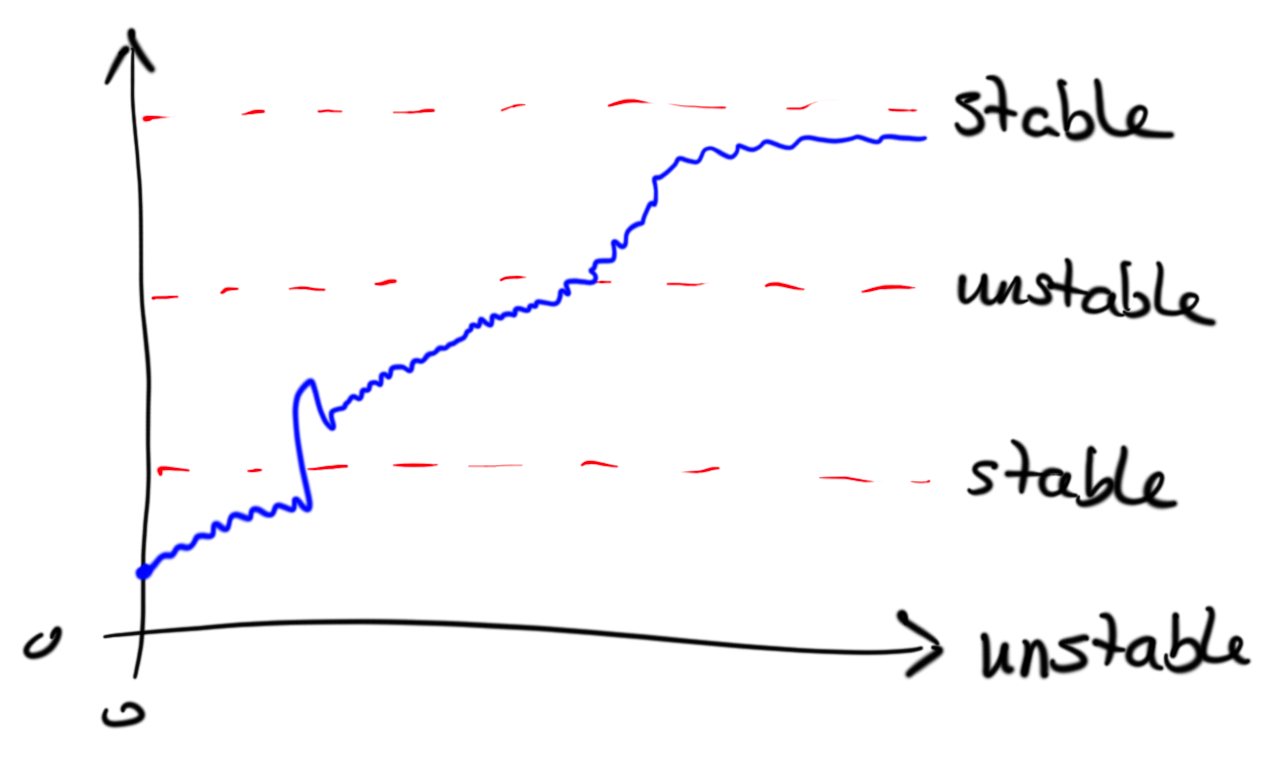
\includegraphics{./figures/L6.1}
\caption{Noise on a trajectory}
\end{figure}
